\documentclass[11pt]{article}
\usepackage[utf8]{inputenc}
\usepackage[italian]{babel}
\usepackage{amssymb}
\usepackage{verbatim}
\usepackage{amsfonts}
\usepackage{amsmath}
\usepackage{amsthm}
\usepackage{xcolor}
\usepackage{graphicx}
\usepackage{float}
\usepackage{enumitem}
\usepackage{fourier} %per il simbolo di Attenzione!
\usepackage{multirow} % Required for multirows
\graphicspath{ {./images/} }

\title{Linguaggi di Programmazione}
\author{Daniele De Micheli}
\date{2019}

\renewcommand*\contentsname{\textit{Indice}}

%presettaggio per teoremi e assiomi/definizioni%

\newtheorem{horn}{Clausole di Horn}
\newtheorem*{isoscele}{Teorema del triangolo isoscele}


%fine%

\begin{document}

\maketitle
\tableofcontents

\part{Introduzione alla logica}
\section{Logica e Ragionamento}
Per poter iniziare a parlare di \textit{linguaggi logici}, dobbiamo prima acquisire cosa è un \textit{linguaggio}.
Dobbiamo quindi capire come un \color{red} ragionamento \color{black} può essere \color{red} formalizzato \color{black} in un numero di \color{red} passi \color{black} (connessi da \color{red} regole \color{black}) a partire da \color{red} premesse \color{black} per raggiungere una \color{red} conclusione \color{black}. 

Questo processo è quello che siamo abituati a riscontrare nella soluzione di \textit{teoremi} tramite \textbf{dimostrazioni}.

Un esempio di applicazione di questo processo possiamo vederlo qui di seguito: 

\begin{isoscele}
Dato un triangolo isoscele, ovvero con due lati $AB = BC$, si dimostra che gli angoli $\angle A$ e $\angle C$ sono uguali.
\end{isoscele}

\textit{\textbf{Conoscenze pregresse}}
\begin{enumerate}
	\item Se due triangoli sono uguali, i due triangoli hanno lati e angoli uguali.
	\item Se due triangoli hanno due lati e l'angolo sotteso uguali, allora i due triangoli sono uguali.
	\item BH bisettrice di $\angle B$ cioè $\angle ABH = \angle HBC$.
\end{enumerate}

\textit{\textbf{Dimostrazione}}
\begin{itemize}
	\item $AB = BC$ per ipotesi;
	\item $\angle ABH = \angle HBC$ per (3);
	\item Il triangolo $HBC$ è uguale al triangolo $ABH$ per (2);
	\item $\angle A \medspace e \medspace \angle C$ per (1); 
\end{itemize}
Quindi abbiamo trasformato (2) in "\textbf{Se} $AB = BC$ e $BH = BH$ e $\angle ABH = \angle HBC$, \textbf{allora} il triangolo $ABH $ è uguale al triangolo $HBC$" e abbiamo trasformato (1) in "\textbf{Se} triangolo $ABH$ è uguale al triangolo $HBC$, \textbf{allora} $AB = BC $ e $ BH = BH $ e $AH = HC $ e $\angle ABH = \angle HBC $ e $\angle AHB = \angle CHB$ e $\angle A = \angle C$".

L'obiettivo diventa a questo punto formalizzare e razionalizzare il processo che permette di affermare $$ AB=BC\vdash\angle A = \angle C$$ dove $\vdash$ indica il simbolo di \color{red} \textit{derivazione logica} \color{black}, che comunemente significa "\textbf{consegue}", "\textbf{allora}", ecc.
\\ \\
\textit{\textbf{Formalizzazione}}
\\ \\
Abbiamo assunto che:
\begin{itemize}
\item $\textbf{P} = \{AB=BC, \angle ABH = \angle HBC, BH = HB\}$.
\end{itemize}
Avevamo inoltre delle conoscenze pregresse (vedi \textit{conoscenze pregresse} sopra riportate).
Abbiamo quindi costruito una catena di \textbf{formule}:
\begin{table}[ht]
  \begin{center}
    \caption{Triangolo Isoscele.}
    \label{tab:isoscele}
    \begin{tabular}{l|l}
      \textbf{Formule} & \textbf{Origine} \\
      \hline
      \multirow{2}{*}{P1:$AB=BC$} 	& da \textbf{P} \\ % <-- Combining 2 rows with arbitrary with (*) and content 12
      								& 10.1 \\ % <-- Content of first column omitted.
      \hline
      P2: $\angle ABH = \angle HBC$  & da \textbf{P} \\
      \hline
      P3: $BH = HB$ &  da \textbf{P}  \\
      \hline
      \multirow{2}{*}{P4:$AB = BC \wedge BH = HB \wedge \angle ABH = \angle HBC$ } 	& da \textbf{P1}, \textbf{P2}, \textbf{P3} e \\ % <-- Combining 2 rows with arbitrary with (*) and content 12
      																				& \color{red} introduzione della congiunzione \color{black} \\
      \hline
      P5: $\bigtriangleup ABH = \bigtriangleup HBC$ & da \textbf{P4}, $regola_{1}$ e \color{red} Modus Ponens \color{black} \\ 
      \hline
      P6:$AB = BC \bigwedge BH = BH \bigwedge AH =HC $ \\ $\medspace \medspace \bigwedge \angle ABH = \angle HBC \bigwedge \angle AHB = \angle CHB \bigwedge $ \\ $\medspace \medspace  \angle A = \angle C$	& da \textbf{P5}, $regola_2$  e \color{red} Modus Ponens \color{black}  \\
      \hline
      \multirow{2}{*}{P7: $\angle A = \angle C$} & da \textbf{P6} e l'\color{red}eliminazione della \\ &\color{red} congiunzione\color{black} (il simbolo $\bigwedge$)
    \end{tabular}
  \end{center}
\end{table}\textbf{•}
\\ \\
Le parti evidenziate in rosso nella tabella \ref{tab:isoscele} sono le \emph{regole di inferenza}.

\subsection{Processo di dimostrazione}
Una "prova" D, dove \color{red}\textbf{S} \color{black} è l'insieme delle \textit{"affermazioni note"} e \textbf{F} la frase (es. la formula) che vogliamo provare.
\begin{equation*}
D\equiv \color{red}\textbf{S}\color{black} \vdash F
\end{equation*} 
(che si legge: \textbf{F} è una conseguenza di \color{red}\textbf{S}\color{black}) è una sequenza di passi $$D = < P_1, P_2, ... , P_n >$$ dove 

$$P_n = F$$  
$$P_i \in S \cup \{P_j \medspace | \medspace j < i\}$$
o $P_i$ può essere ottenuto da $P_{i1},...,P_{im}$ (con $i1 < i, ... , im < i$)mediante l'applicazione di una regola di inferenza.

\subsection{Regole di inferenza e calcoli logici}
Un insieme di regole di inferenza costituisce la base di un calcolo logico. Diversi insieme di regole danno vita a diversi calcoli logici. Lo scopo di un calcolo logico è quello di manipolare delle formule logiche in modo completamente \textbf{sintattico} al fine di stabilire una
connessione tra un insieme di formule di \textit{partenza} (di solito un
insieme di formule dette \emph{assiomi}) ed un insieme di \textit{conclusioni}.

\section{Programmazione Logica}
La programmazione logica nasce all'inizio degli anni settanta da
studi sulla deduzione automatica: il \textit{\textbf{Prolog}} costituisce uno dei
sui risultati principali. Essa non è soltanto rappresentata dal Prolog; costituisce infatti un settore molto ricco che cerca
di utilizzare la logica matematica come base dei linguaggi di
programmazione.
\\ \\ 
Gli obiettivi del linguaggio di programmazione logica sono:
\begin{itemize}
	\item semplicità del formalismo;
	\item linguaggio ad alto livello;
	\item semantica chiara;
\end{itemize}
Questo tipo di linguaggio si focalizza sulle solide basi della \textit{logica matematica}. Con l'avvento dell'informatica difatti si è sempre più utilizzata la logica matematica per dimostrare teoremi tramite i calcolatori (che permettono di ottenere risultati in minor tempo e con meno errori). Tra le procedure utilizzate si ricordano la \textit{procedura di Davis e Putnam} e il \textit{principio di risoluzione}. 

Per rendere bene l'idea, la programmazione logica viene utilizzata per verificare la correttezza di altri software, per rappresentare la conoscenza di Intelligenza Artificiale o ancora per il formalismo nei database (come Datalog).

\subsection{Stile dichiarativo della programmazione logica}
Lo stile della programmazione logica ha delle precise caratteristiche:
\begin{itemize}
 	\item[$\circ$] Un programma è un \textit{insieme di formule}.
 	\item[$\circ$] Possiede un grande potere espressivo.
 	\item[$\circ$] Il processo di risoluzione prevede la costruzione di una dimostrazione logica di un'affermazione (\textbf{goal}).
 	\item[$\circ$] Possiede una \color{red}base formale\color{black}:
 	\begin{itemize}
 		\item[--] Calcolo dei predicati del primo ordine (vedi sez. ????) ma con limitazione nel tipo di formule (\textbf{\emph{clausole di Horn}} (\ref{thm:horn}))
 		\item[--] Utilizzo di particolari tecniche per la dimostrazione di teoremi (meccanismo di \textbf{\emph{Risoluzione}})
 	\end{itemize}
\end{itemize}

\subsection{PROLOG}
Il Prolog (acronimo di \textbf{PRO}gramming in \textbf{LOG}ic) fu ideato e realizzato nel 1973 da Robert Kowalski (aspetto teorico) e Marten Van Emdem (dimostrazione sperimentale) . Esso si basa su una restrizione della \textit{logica del primo ordine}. Come caratteristica base dei linguaggi logici, anche Prolog utilizza uno stile dichiarativo di programmazione. La sua primaria funzione è quella di determinare se una certa affermazione è vera oppure no e, se è vera, quali vincoli sui valori attribuiti alle variabili hanno generato la risposta.


\paragraph{Formule ben formate} Le formule ben formate (\textit{fbf}, o \textbf{well-formed formula}, \textit{wff}) di un linguaggio logico del primo ordine può essere riscritta in \color{red}forma normale a clausole\color{black}.

Vi sono due forme normali a clausole:
\begin{itemize}
	\item[$\circ$]\color{blue}Forma normale congiunta\color{black} (conjunctive normal form - CNF): la formula è una \textbf{congiunzione} di \textbf{disgiunzioni} di predicati o di negazioni di predicati (letterali \textit{positivi} o letterali \textit{negativi}).
	\begin{equation}
	\label{eqz:CNF}
	\bigwedge_i \bigg( \bigvee_j L_{ji} \bigg) 
	\end{equation}
	\item[$\circ$]\color{blue}Forma normale disgiunta\color{black} (disjunctive normal form - DNF): la formula è una \textbf{disgiunzione} di \textbf{congiunzioni} di predicati o di negazione di predicati (letterali \textit{positivi} o letterali \textit{negativi}).
	\begin{equation}
	\bigvee_j \bigg( \bigwedge_i L_{ji} \bigg) 
	\end{equation}
\end{itemize}
dove 
\begin{equation*}
	L_{ij} \equiv P_{ij} (x,y,...,z) \circ L_{ij} \equiv \neg Q_{ij}(x,y,...,z)
\end{equation*}

\subsubsection{Forma Normale Congiuntiva}
Consideriamo una \textit{wff} in CNF (\ref{eqz:CNF}). Per esempio:
\begin{equation}
\label{eqz:es1CNF}
\underbrace{(p(x) \vee q(x,y) \vee \neg t(z))}_{clausola \medspace 1} \color{red}\wedge\color{black} \underbrace{(p(w) \vee \neg s(u) \vee \neg r(v)}_{clausola \medspace 2})
\end{equation}
se scartiamo il simbolo di \color{red}congiunzione \color{black}  (\ref{eqz:es1CNF}), rimaniamo con solo le clausole disgiuntive
\begin{enumerate}
	\item $(p(x) \vee q(x,y) \vee \neg t(z))$
	\item $(p(w) \vee \neg s(u) \vee \neg r(v))$
\end{enumerate}
Le clausole così ottenute sono anche riscrivibili come
\begin{enumerate}
	\item $t(z) \Rightarrow p(x) \vee q(x,y)$ 
	\item $s(u) \wedge r(v) \Rightarrow p(w)$
\end{enumerate}
ovvero un insieme di formule in CNF è riscrivibile come un insieme (congiunzione) di implicazioni.

\begin{horn}
\label{thm:horn}
Le clausole che hanno al più un solo letterale positivo (con o senza letterali negativi) prendono il nome di \textbf{\emph{Clausole di Horn}}.
\end{horn}
Detto questo, abbiamo che:
\begin{itemize}
	\item Non tutte le fbf possono essere trasformate in un insieme di clausole di Horn.
	\item \textit{I programmi Prolog sono collezioni di clausole di Horn}
\end{itemize}

\subsubsection{Struttura del Prolog}
Il linguaggio Prolog:
\begin{itemize}
	\item[$\circ$]Non contiene (quasi) istruzioni
	\item[$\circ$]Contiene solo fatti e regole (clausole di Horn):
	\begin{itemize}
		\item \textbf{Fatti}: asserzioni vere nel contesto che stiamo descrivendo.
		\item \textbf{Regole}: ci danno gli strumenti per dedurre nuovi fatti da quelli esistenti.
	\end{itemize}
	\item[$\circ$]Un programma Prolog ci dà informazioni su un sistema ed è normalmente chiamato \color{red}base di conoscenza \color{black}(\color{red}knowledge base\color{black})
	\item[$\circ$]Un programma Prolog non si "esegue" ma si \textit{"interroga"} (\textbf{queried}): al programma si chiede se i fatti sono veri; esso risponderà son un \color{blue}True \color{black} o \color{blue}False \color{black} alla domanda.
\end{itemize}

\subsubsection{Sintassi del Prolog}
Un programma Prolog è costituito da un insieme di clausole della forma


\begin{table}[ht] %ht indica di creare la tabella dove la metti, sempre che sia possibile.
	\begin{center}
	\caption{Sintassi Prolog}
	\label{sintassiProlog}
	\begin{tabular}{l|l}

	$a.$ & \color{red}FATTO / ASSERZIONE\color{black} \\
	\hline
	$c :- \medspace b_1 , b_2 , _ , b_n . $ & \color{red}REGOLA\color{black} \\
	\\ \\

	$:- \medspace q_1 , q_2 , ... , q_m $ & \color{red}GOAL\color{black} \\
	\hline
	$?-\medspace q_1 , q_2 , ... , q_m $ & \color{red}QUERY\color{black} \\
	
	
	\end{tabular}
	\end{center}
\end{table}
In cui $a, b_i \medspace e \medspace  q_i $ sono \emph{\textbf{termini}} (compositi). 
Da notare che in molte implementazioni il prompt Prolog è un operatore che chiede al sistema di valutare il \textbf{goal}, in questo caso una congiunzione di termini. 
\paragraph{Termini} Le espressioni nel Prolog sono chiamate \color{red}\textbf{termini}\color{black}. Esistono diversi tipi di termini:
\begin{itemize}
	\item[$\circ$]ATOMI :
	\begin{itemize}
	
	\item Una sequenza di caratteri alfanumerici, che inizia con un carattere minuscolo (può contenere il carattere $"_"$ underscore)
	\item Qualsiasi cosa racchiusa tra apici singoli (' ')
	\item Un numero
	\item Una stringa (SWI Prolog)
\end{itemize}
	\item[$\circ$]VARIABILI:
	\begin{itemize}
	
	\item Una variabile (logica) è una sequenza alfanumerica che inizia con un carattere \textbf{MAIUSCOLO} o con il carattere $\_$ (underscore)
	\item Le variabili (notare il plurale) composte solo dal simbolo $\_$ sono chiamate \textbf{indifferenza} (\textit{don’t care o any}) o \textbf{anonime}
	\item Le variabili vengono \textbf{istanziate} (legate a un valore) con il
procedere del programma (nella dimostrazione del teorema)
\end{itemize}
	\item[$\circ$]Una composizione di termini $\Rightarrow$ TERMINE COMPOSTO (simbolo di \color{red}\textit{funtore} \color{black} più uno o due argomenti):
	\begin{itemize}
		\item[+] Un \textbf{funtore} (simbolo di funzione o di predicato definito come atomo)
		\item[+] Una sequenza di termini racchiusi tra parentesi tonde e
separati da virgole. Questi sono chiamati argomenti del funtore
	\end{itemize}
	
\end{itemize}
%\danger \leaders\vrule height 2.5pt depth -1.5pt \hfill \null
%\\ \\
\danger\medspace\danger \hfill \danger\medspace\danger
\\ \\
\textbf{\emph{Non ci deve mai essere uno spazio tra il funtore e la parentesi di
sinistra}}; questo per via di caratteristiche molto sofisticate del
sistema di parsing di Prolog (cfr., operatori)
\\ \\
\danger\medspace\danger \hfill \danger\medspace\danger
\\ \\
\paragraph{Prolog: fatti e predicati}

Un \textbf{fatto} (\textbf{predicato}) consiste in:
\begin{itemize}
	\item Un nome di predicato, ad esempio \textit{fattoriale}, \textit{genitore}, \textit{uomo} o \textit{animale}; deve iniziare con una lettera \color{red} minuscola\color{black}.
	\item Zero o più argomenti come \textit{maria}, \textit{42} o \textit{cane}. Da tenere presente che i fatti (e le regole e le domande) \textbf{devono} essere terminati da un punto (".").
\end{itemize}

\paragraph{Le regole} In Prolog si usano le \textbf{regole} quando si vuole esprimere che un certo fatto dipende da un insieme di altri fatti. Per esprimere in linguaggio naturale questa dipendenza usiamo la parola "\color{blue}se\color{black}" ("if" in inglese).

Ad esempio:
\begin{itemize}
	\item \textit{Uso l'ombrello \textbf{se} piove};
	\item \textit{Luca mangia la pizza \textbf{se} non contiene glutine};
\end{itemize}
Le regole sono anche usate per esprimere definizioni. Ad esempio:
\subparagraph{X è un pesce \textbf{se}:}
\begin{itemize}
	\item X è un animale
	\item X ha le squame
\end{itemize}
Una regola è costituita da una \color{blue}\textbf{testa }\color{black} e da un \color{blue}\textbf{corpo}\color{black}. Sono inoltre caratterizzati come segue:
\begin{enumerate}
	\item Testa e corpo sono collegati dalloperatore "$:-$".
	\item La testa di una regola corrisponde al \color{red}\textbf{conseguente} \color{black} di un'implicazione logica. 
	\item Il corpo di una regola corrisponde all’\color{red}\textbf{antecendente} \color{black} di un’implicazione logica.
	\item Le regole Prolog corrispondono alle \color{blue}\textbf{clausole di Horn} \color{black}, ovvero hanno un solo termine (predicato) come conseguente.
	\begin{itemize}
		\item[$\circ$] L'operatore Prolog '$:-$' esprime il "\textbf{se}" (\textit{implicazione}).
		\item[$\circ$] L'operatore Prolog ',' equivale a "\textbf{e}" (\textbf{\textit{and}}, o \textit{congiunzione}).
	\end{itemize}
\end{enumerate}
Un esempio di regola Prolog può essere:
\\ \\
\textit{"un pesce è un animale che ha le squame"} diventa:
\begin{flalign}
& pesce(X) \medspace :- \medspace animale(X), \medspace ha\_ le\_ squame(X). && \nonumber 
\end{flalign}
Una relazione può essere però definita per necessità da due regole (o clausole) aventi lo stesso predicato come conclusione. Per esempio:
\begin{flalign*}
&genitore(X, Y) \medspace :- \medspace padre(x, Y). && \\\nonumber
&genitore(X, Y) \medspace :- \medspace madre(x, Y). &&
\end{flalign*}
Le regole (ed i fatti) sono implicitamente connesse dall'operatore logico di congiunzione ("\color{red}and\color{black}"); se non si sono commessi errori logici, \textbf{entrambe} le implicazioni soprastanti sono da ritenersi \textbf{vere}.
\\ \\
Una relazione può essere definita anche \emph{ricorsivamente}. In questo caso la definizione richiede almeno due proposizioni: una è quella ricorsiva che corrisponde al caso generale, l'altra esprime il caso base più semplice.

\begin{flalign*}
&antenato(X, Y) \medspace :- \medspace genitore(X,Y). &&\\\nonumber
&antenato(X, Y) \medspace :- \medspace genitore(Z,Y), antenato(X, Z).&&
\end{flalign*}

\subparagraph{Operatori Logici}: gli operatori logici "and" e "or" possono essere utilizzati nelle regole tramite una specifica sintassi.
L'operatore "\textbf{AND}" viene inserito in una regola con il carattere \textit{virgola} ',';
L'operatore "\textbf{OR}" viene inserito in una regola con il carattere  \textit{punto e virgola} ';'.

\subparagraph{RICAPITOLANDO} Bisogna ricordare che:
\begin{enumerate}
	\item ogni fatto o regola DEVE terminare con un punto '.'
	\item ogni variabile DEVE iniziare con una MAIUSCOLA
	\item i commenti si inseriscono dopo un "\%" (commento in linea) o tra '/*' e '*/' (come in altri linguaggi).
\end{enumerate}

\subsubsection{Modello di esecuzione}
Come abbiamo già visto, il Prolog utilizza un'interpretazione dichiarativa. Per esempio, 
\begin{equation}
p:-q,r.
\end{equation}
si può leggere come "\textit{p è vero se sono veri q e r}".
Abbiamo anche una interpretazione procedurale, in cui il problema $p$ viene scomposto nei sottoproblemi $q$ e $r$. In questa visione, un \textit{goal} può essere visto come una chiamata ad una procedura in cui la testa è l'intestazione mentre la parte destra è il corpo.

\paragraph{Controllo di esecuzione} Come abbiamo abbiamo intuito, le clausole nel data base di un programma Prolog vengono considerate "da sinistra, verso destra" e "dall’alto al basso". Se un (sotto)goal fallisce, allora il dimostratore Prolog sceglie un'alternativa, scandendo "dall'alto verso il basso" la lista delle clausole (nella pratica, esegue in ordine le istruzioni che trova). 

Per poter manipolare l'esecuzione, il Prolog dispone di un \textit{predicato} speciale, chiamato \color{red} cut \color{black} (\textit{taglio}, scritto con il solo simbolo esclamativo "!"). Le principali caratteristiche del \textbf{cut} sono le seguenti:
\begin{itemize}
	\item Il cut è molto complesso da interpretare (non ha un'interpretazione logica ma bensì procedurale);
	\item La sua importanza non può essere sottovalutata; è un predicato potente, difficile da usare nel modo corretto e particolarmente utile se usato correttamente.
	\item Per capire come funziona è necessario avere un'idea del funzionamento del dimostratore Prolog.
\end{itemize}

\paragraph{Il predicato cut '!'} Consideriamo la seguente clusola generica con \color{red}cut\color{black}:
\begin{equation*}
C= a:-b_1, b_2,...,b_k, \color{red}!\color{black}, b_{k+1}, ..., b_n
\end{equation*}
L'effetto del \textit{cut} è il seguente:
\begin{itemize}
	\item Se il goal corrente unifica con $a$ e $b_1,...,b_k$ hanno successo, allora il dimostratore si impegna inderogabilmente alla scelta di $C$ per dimostrare $G$.
	\item Ogni clausola alternativa (successiva, in basso) per \textit{a} che unifica con \textit{G} viene ignorata.
	\item Se un qualche $b_j$ con $j > k$ fallisse, il backtracking si fermerebbe al \textit{cut}. Le altre scelte per $b_i$ con $i \leqslant k$ sono di conseguenza rimosse dall'albero di derivazione.
	\item Quando il backtracking raggiunge il \textit{cut}, allora il \textit{cut} fallisce e la ricerca procede dall'ultimo punto di scelta prima che \textit{G} scegliesse \textit{C}.
\end{itemize}

Qui di seguito è proposto un esempio di goal e di clausole contenente il \textit{cut} e di cui viene mostrato l'albero di derivazione.

\begin{figure}[H]
\label{Albero sintattico che mostra il funzionamento del predicato cut}
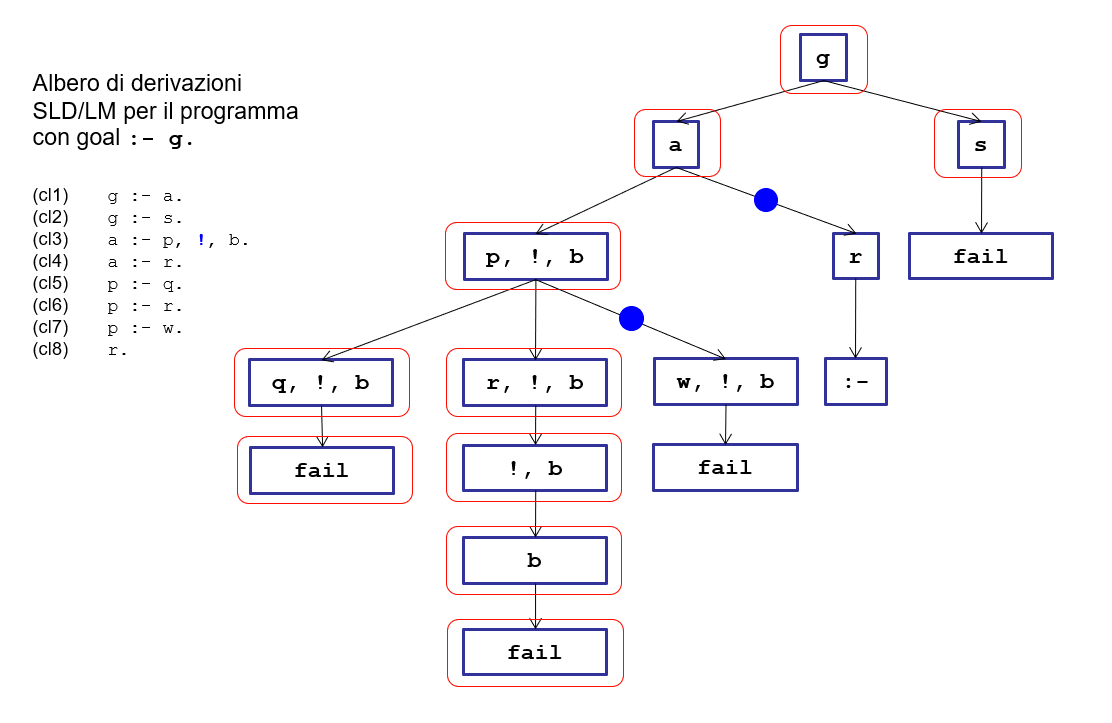
\includegraphics[scale=0.35]{cut-albero-derivazioni.png}
\centering
\end{figure}

Nella figura si può notare il percorso di dimostrazione che l'interprete Prolog segue. Si può anche notare che tra i percorsi "tagliati" fuori dal risultato (quelli posti dopo il pallino blu nel collegamento tra padre e figlio) c'è pure l'unico \textbf{successo} possibile della query rispetto alle clausole di programma. In questo caso infatti possiamo dire che il \textit{cut} ha escluso la soluzione dai risultati.

\subsection{L'interprete Prolog: interrogazioni}
Una volta che le regole e i fatti sono stati "caricati" nell'interprete, eseguire un programma Prolog equivale a \textit{interrogare} l'\textbf{interprete}. Una volta fatto partire, l'interprete Prolog ci presenta un prompt così:
\begin{flalign*}
& ?- &&\nonumber
\end{flalign*}
Come si può intuire anche dalla sintassi del prompt, interrogare l'interprete non è altro che porre una \textit{domanda} a cui generlamente il Prolog risponde "\textbf{true}" o "\textbf{false}".
Le interrogazioni possono contenere variabili interpretate come \emph{\textbf{variabili esistenziali}}. Queste sono istanziate quando il Prolog prova a rispondere alla domanda fattagli. Tutte le variabili istanziate vengono mostrate nella risposta insieme a "true".

\subsubsection{L'interprete prolog: \textbf{consult}}
Nel Prolog la base di conoscenza è \textit{nascosta} ed è accessibile solo tramite opportuni comandi o tramite ambiente di programmazione. Ovviamente è necessario poter \emph{inizializzare} o \emph{caricare} un insieme di fatti e regole nell'ambiente Prolog.
Il comando principale che assolve questa funzione è \textbf{consult}:
\begin{itemize}
	\item Il comando consult appare come un predicato da valutare (un goal) e prende
almeno un termine che denota un file come argomento.
	\item Il file deve contenere un insieme di fatti e regole.
\end{itemize}

\subsubsection{Risoluzione ad Input Lineare}
Il sistema Prolog dimostra la veridicità o meno di un'interrogazione (un goal) eseguendo \textit{una sequenza di passi di risoluzione}. L'ordine complessivo in cui questi passi vengono eseguiti rende i sistemi di prova di teoremi basati su risoluzione più o meno "\emph{efficaci}".

Infatti, in Prolog la risoluzione avviene sempre tra l'ultimo goal derivato in ciascun passo e una "clausola di programma"; non avviene mai tra due clausole di programma o fra una clausola di programma ed un goal derivato in precedenza. 
Questa particolare forma di risoluzione prende il nome di \color{blue} Risoluzione SLD \color{black} (\textit{Selection} function for \textit{Linear} and \textit{Definite} sentences \textbf{Resolution}) in cui le frasi "lineari" sono essenzialmente le clausole di Horn.
\\ \\
Questo metodo di risoluzione funziona in modo semplice ed efficace. Prendiamo ad esempio il seguente goal $G_j$:
\begin{equation}
G_j \equiv ?- A_{i,1}, \: A_{i,2}, \: A_{i,3},...,A_{i,m}.
\end{equation}
e la regola 
\begin{equation}
A_r :- B_{r,1}, B_{r,2}, ...,B_{r,k}.
\end{equation}
se esiste un unificatore $\sigma$ tale che $\sigma [A_r] = \sigma [A_{i,1}]$, allora si ottiene un nuovo  goal $G_{j+1}$
\begin{equation}
G_{j+1} \equiv ?- B^1_{r,1}, B^1_{r,2}, ... ,B^1_{r,k}, A^1_{i, 2},A^1_{i, 3},...,A^1_{i, m}.
\end{equation}
Questo è \textbf{un} passo di risoluzione eseguito dal sistema Prolog (in cui $A^1$ e i $B^1$ sono i risultati $\sigma [A] = A^1$ e $\sigma [B] = B^1$.
In altre parole, potremmo scrivere l'esempio come sequenza di passaggi:
\begin{enumerate}[label=(P\arabic*)]
	\item $A_r (=A_{i,1}) :- \neg B_1 \wedge B_2 \wedge ... \wedge B_n$
	\item $\neg A_{i,1} \vee \neg A_{i,2} \vee ... \vee \neg A_{i,m}$
	\item $A_{1,1}, \vee \neg B_1 \vee \neg B_2 \vee ... \vee \neg B_n$
	\item $\neg B_1 \vee \neg B_2 ... \vee \neg B_n \vee \neg A_{i,2} \vee \neg A_{i,3} ... \vee \neg A_{i,m} $
\end{enumerate}
Noi sappiamo che $A_{i,1}$ può essere risolto con $A_r$. Ma $A_r$ è a sua volta una query (P1). Il primo termine della query può essere unificato con il negato della seconda, il quale produce il nuovo goal (P4).
\\ \\
In una soluzione SLD, il passo di risoluzione avviene sempre tra l'ultimo goal e una clausola di programma. Il risultato può essere
\begin{itemize}
	\item SUCCESS: viene generata la clausola vuota, ovvero se per  finito, $G_n$ è uguale alla clausola vuota $G_n \equiv :- $
	\item FINITE INSUCCESS: se per $n$ finito, $G_n$ non è uguale alla clausola vuota e non è più possibile derivare un nuovo \textit{risolvente} da $G_n$ ed una clausola di programma.
	\item INFINITE INSUCCESS: se è possibile derivare nuovi \textit{risolventi} tutti diversi dalla clausola.
\end{itemize}
Durante il processo di generazione di goal intermedi si costruiscono delle variabili dei letterali e delle clausole coinvolti mediante la rinominazione di variabili.
La rinominazione avviene nel momento in cui si genera un nuovo goal ma ci si deve portare dietro le variabili che non sono state unificate, per esempio. 

Un esempio di \textbf{renaming} di variabili è il seguente: presa
$$p(X) :- q(X, g(z)). $$
è equivalente alla clausola 
$$p(X1) :- q(X1, g(FooFrobboz)). $$
rinominata.
\\ \\
Per applicare la risoluzione del goal corrente ci possono essere diverse clausole di programma adeguate al compito. Ci sono diverse strategie, di cui due sono le seguenti:
\begin{enumerate}
	\item \textbf{In profondità (\textit{Depth First}}: si sceglie una clausola e si mantiene fissa questa scelta, finché non si arriva alla clausola vuota o alla impossibilità di fare nuove risoluzioni; in questo ultimo caso si riconsiderano le scelte fatte precedentemente.
	\item \textbf{In ampiezza (\textit{Breadth First}}: si considerano in parallelo tutte le possibili alternative.
\end{enumerate}
Il Prolog adotta una strategia di risoluzione "\textit{in profondità}" con \color{blue} backtracking\color{black}. Questo permette di risparmiare memoria ma non è completa per le clausole di Horn.

\subsubsection{Alberi di derivazione SLD}
Dato un programma logico $P$, un goal $G_0$ e una regola di calcolo $R$, un \textbf{albero SLD} per $P \cup \{G_0\}$ via $R$ è definito sulla base del processo di prova visto precedentemente;
\begin{itemize}
	\item Ciascun nodo dell'albero è un goal (possibilmente vuoto)
	\item La radice dell'albero SLD e il goal $G_0$
	\item Dato il nodo 
		\begin{equation*}
		:- A_1 , ... ,A_{m-1}, A_m, A_{m+1},...,A_k.
		\end{equation*}
		se $A_m$ è il sottogoal \textit{selezionato} dalla regola di calcolo $R$, allora questo nodo (genitore) ha un nodo figlio per ciascuna clausola del tipo
		\begin{flalign*}
		& C_i \equiv A_i :- B_{i,1}, ... ,B_{i, q}&&\\\nonumber
		& C_k \equiv A_k. &&
		\end{flalign*}
		di P tale che $A_i$ e $A_m$  ($A_k$ e $A_m$) sono unificabili attraverso la sostituzione più generale $\sigma$.
		\item Il nodo figlio è etichettato con la clausola goal 
		\begin{flalign*}
		& :- \sigma [A_1, ... , A_{m-1}, B_{i,1}, ... , B_{i,q}, A_{m+1}, ... A_k]&&\\\nonumber
		& :- \sigma [A_1, ... , A_{m-1}, A_{m+1}, ... A_k] &&
		\end{flalign*}
		e il ramo dal nodo padre al figlio è etichettato dalla sostituzione $\sigma$ e dalla clausola delezionata $C_i$ (o $C_k$).
		\item Il nodo vuoto (indicato con ":-") non ha figli.
\end{itemize}

\subsection{Unificazione}
L'operazione di istanziazione di variabili durante la "prova" di un
predicato è il risultato di una procedura particolare, detta
unificazione. Dati due termini, la procedura di unificazione crea un insieme di \emph{sostituzioni} delle variabili, il quale permette di rendere "\textbf{uguali}" i due termini.
\\ \\
Tradizionalmente la procedura di unificazione costruisce un insieme di
sostituzioni chiamato "\color{blue}most general unifier\color{black}" ed indicato con \textit{Mgu}. Una sostituzione è indicata come una sequenza (ordinata) di coppie variabile/valore.

Esempi:
\begin{flalign*}
& Mgu(42, 42) \qquad \qquad \qquad \qquad \qquad \qquad \Rightarrow \{ \}&&\\\nonumber
& Mgu(42, X) \medspace \medspace \qquad \qquad \qquad \qquad \qquad \qquad \Rightarrow \{X/42\}&&\\\nonumber
& Mgu(X, 42) \medspace \medspace \qquad \qquad  \qquad \qquad \qquad \qquad \Rightarrow \{X/42\}&&\\\nonumber
& Mgu(foo(bar, 42), foo(bar, X)) \quad \medspace \medspace \medspace \medspace \medspace \quad \Rightarrow \{X/ 42\}&&\\\nonumber
& Mgu(foo(Y, 42), foo(bar, X)) \quad \medspace\medspace \medspace \medspace \medspace \qquad \Rightarrow \{X/ 42\}&&\\\nonumber
& Mgu(foo(X), foo(bar(Y))) \quad\quad \medspace\medspace \medspace \medspace \medspace \qquad \Rightarrow \{X/bar(Y), Y/\_ G001\}&&\\\nonumber
\end{flalign*}
Notare l'ultimo esempio con \textbf{ridenominazione} di variabili (\_ G001 è il nome assegnato alla variabile che contiene il risultato. Esso è generato dal programma Prolog).
Il "\textit{most general unifier}" non è nient'altro che il risultato finale della procedura di valutazione - ovvero di prova - del Prolog. 

Il modo più semplice per vedere come la procedura di unificazione funziona è di
usare l'operatore Prolog = (detto, per l'appunto, \color{blue}operatore di unificazione\color{black}).
\\ \\
Esempi:
\begin{flalign*}
&?- \quad \textbf{42 = 42.} &&\\\nonumber
& \quad\quad Yes &&\\\\\nonumber
&?- \quad \textbf{42 = X.} &&\\\nonumber
& \quad \quad X=42&&\\\nonumber
& \quad \quad Yes&&\\\\\nonumber
&?- \quad \textbf{foo(Y, 42)=foo(bar, X).} &&\\\nonumber
& \quad \quad Y=bar&&\\\nonumber
& \quad \quad X=42&&\\\nonumber
& \quad \quad Yes&&\\\\\nonumber
\end{flalign*}

\subsection{Liste in Prolog}
Si definisce una \textit{lista} in Prolog racchiudendo gli elementi (termini
e/o variabili logiche) della lista tra parentesi quadre
'[' e ']' e separandoli da virgole. Gli elementi di una lista in Prolog possono essere termini qualsiasi o liste. Per indicare una lista vuota si usa la notazione '[ ]'.
\\ \\
Ogni lista non vuota può essere divisa in due parti, una \color{red}\textit{testa} \color{black} ed \color{red}\textit{coda} \color{black}:
\begin{itemize}
	\item La \color{red}\textit{testa} \color{black} è il primo elemento della lista.
	\item La \color{red}\textit{coda} \color{black} rappresenta tutto il resto della lista ed è \textbf{SEMPRE} una lista.
\end{itemize}


\subsubsection{L'operatore | }
Prolog possiede uno speciale operatore usato per distinguere tra l'inizio e la coda di una lista: l'operatore "\textbf{|}".

Esempi dell'operatore | :
\begin{flalign*}
&?- \quad \textbf{[X | Ys] = [mia, vincente, jules, yolanda].} &&\\\nonumber
& \quad \quad X=mia&&\\\nonumber
& \quad \quad Ys=[vincent, jules, yolanda]&&\\\nonumber
& \quad \quad Yes&&\\\\\nonumber
&?- \quad \textbf{[X, Y | Zs] = [the, answer, is, 42].} &&\\\nonumber
& \quad \quad X=the&&\\\nonumber
& \quad \quad Y=answer&&\\\nonumber
& \quad \quad Zs=[is, 42]&&\\\nonumber
& \quad \quad Yes&&\\\\\nonumber
&?- \quad \textbf{[X, 42 | \_] = [41, 42,43, foo(bar)].} &&\\\nonumber
& \quad \quad X=41&&\\\nonumber
& \quad \quad Yes&&\\\\\nonumber
\end{flalign*}



\end{document}
